\documentclass[conference]{IEEEtran}
\IEEEoverridecommandlockouts
% The preceding line is only needed to identify funding in the first footnote. If that is unneeded, please comment it out.
\usepackage{cite}
\usepackage{amsmath,amssymb,amsfonts}
\usepackage{algorithm}
\usepackage{algorithmic}
\usepackage{graphicx}
\usepackage{textcomp}
\usepackage{xcolor}
\usepackage{multirow}
\usepackage{multicol}
\usepackage{subfigure}
\usepackage{ntheorem}
\usepackage{enumerate}
\usepackage[bottom]{footmisc}
\usepackage{soul}

\usepackage[T1]{fontenc}
\usepackage{mathptmx}
\soulregister\cite7
\soulregister\ref7
\pagestyle{plain}

\def\BibTeX{{\rm B\kern-.05em{\sc i\kern-.025em b}\kern-.08em
    T\kern-.1667em\lower.7ex\hbox{E}\kern-.125emX}}
\begin{document}

\title{\LARGE{Approximate Code: A Cost-Effective Erasure Code for MultimediavApplications in Cloud Storage Systems}\\
}
\author{\IEEEauthorblockN{Huayi Jin$^1$}
}

\maketitle

\begin{abstract}
Erasure codes are commonly used to ensure data availability in cloud storage systems, where video data produced by autopilot, multimedia industry and security monitoring occupies large amounts of space. 
Typical erasure codes, such as Reed-Solomon (RS) codes or XOR-based codes use several parity disks to fully recover failure disks. 
However, this is expensive, not only because the scenes in which multiple disks are simultaneously damaged are relatively rare, but also because they do not consider redundant information inside the data, which results in multiple complete parity disks being excessive.   
   

Therefore, we propose Approximate Codes for video data, which significantly reduce storage overhead and increase availability for more important data segments.
Approximate Codes provide complete recovery when fewer disks fail, and approximate recovery (recover most data) in the event of multiple disk failures.
To demonstrate the effectiveness of Approximate Codes, we conduct several experiments in Hadoop and Alibaba Cloud systems.
The results show that compared with the typical high-reliability erasure code schemes, Approximate Codes reduce the storage overhead by 7.64\% at the expense of reasonable probability of video quality loss.

\end{abstract}

\begin{IEEEkeywords}
    Erasure Codes, Approximate Storage, Multimedia, Cloud Storage
\end{IEEEkeywords}

\section{Introduction}
Currently, many cloud storage systems use erasure codes to tolerate disk failures and ensure data availability, such as Windows [], Amazon AWS [] or Alibaba Cloud. It is known that erasure codes provide much lower storage overhead and write bandwidth than replication with the same fault tolerance.

Typical erasure codes schemes can be divided into two categories such as RS-based code (RS, LRC), or XOR-based code (...). Other erasure codes (SD, STAIR) use the parity blocks to tolerate sector failures in addition to disk-level fault tolerance.

Video data consumes massive space in cloud storage systems, and this trend is exacerbated as applications demand increased resolution and frame rates. Using multiple copies to ensure video data security will generate storage cost that are several times larger than the original data, which is obviously too expensive, while erasure codes can significantly reduce this cost.

Existing erasure codes are designed to completely recover corrupted data. Typical configurations use triple disk failure tolerant arrays (3DFTS), such as Windows Azure [], which requires at least 3 parity disks. These methods are often excessive because scenes with 3 disks being corrupted at the same time are very rare as well as they do not consider that plenty of video applications can tolerate a certain amount of data loss. For example, video data typically records at least 20 frames per second, which makes losing a few frames difficult for a typical user to perceive. In addition, even if the video data suffers a certain loss, the existing AI-based interpolation algorithm and super pixel algorithm can recover most of the damaged data [].

We also find that video data is usually stored after being encoded to save space, while the encoded video data stream is non-uniformly sensitive to data loss, which makes it inappropriate to provide uniform fault tolerance using conventional erasure codes. With the motion compensation mechanism, common video coding algorithms such as H.264 only needs to store the complete content of key frames and a little part of other frames, which makes other frames rely on the key frames for computation while decoding.

Therefore, we propose Approximate Codes for video data that significantly reduce storage overhead by reducing the parity of data that is not sensitive to errors. In the scenario shown in (Figure 1), the Approximate Codes are designed for systems composed of $n$ disks where $m$ disks are dedicated to coding and another $s$ sectors encoded for the first strip. This allows the data of the first stripe to tolerate any $m+s$ disks corruption, so we specifically store important segments of video data there. With an appropriate data distribution scheme, non-critical data segments will still retain $(n-2m-s)/(n-m)$ data when any $m+s$ disks are corrupted, which makes 
recovery schemes such as interpolated or superpixel still effective. The approximate codes provide two recovery modes, full recovery and approximate recovery. The former applies to no more than $m$ disk corruptions and recovers all data, the latter applies to no more than $m+$s disks corruptions and retains important data.

\section{Related Work and Our Motivation}
Video data can be classified into hot data and cold data, the former requiring high availability and reliability, which often relies on expensive replication approach. The latter's storage usually uses erasure codes schemes, because cold data far exceeds hot data, and erasure codes can guarantee its reliability with low monetary overhead. However, existing erasure code schemes do not consider the characteristics of video data and are not specifically designed for them.

Videos are typically stored in lossy compression, so they are subject to a certain quality loss when stored compared to the original version, and the extent of this quality loss can be specified by the application. For high-quality coded video, it is difficult for the human eye to distinguish the difference between them and the original video, because they preserve most of the brightness information, which human eye is very sensitive to, and some color information is discarded, which human eye is not sensitive to. Therefore, the encoded video data has an uneven degree of importance, that is, it is tolerable that some of those less important data losses because the users are hard to detect. On the other hand, loss of important data will have more serious consequences.

This section then introduces the relevant background and our motivation.

\subsection{Existing Erasure Codes}
RS/LRC/CLAY/SD/STAIR…
XOR-based
RS-based
RAID6
MSR

\subsection{Approximate Storage}
Approximate Storage loosen the requirement of storage reliability by allowing some quality loss of specific data, which recently receives more attentions since data centers are trading off the limited resource budget with the costly reliability requirements of ever-increasing data.

\subsection{Video Storage}
For normal HD (resolution 1280$\times$720, 8-bit, 30 fps) video, the amount of raw video data in 1 minute is 4.63 GB, so video data is usually encoded and compressed before storage. Lossy compression is a common method that provides a much lower compression ratio than lossless compression while ensuring tolerable loss of video quality, so we focus on such algorithms. 

H.264 is one of the advanced algorithms for this type of work. This coding technique is widely used on platforms such as YouTube because it has higher compression ratio and lower complexity than its predecessor. For the HD video mentioned earlier, H.264 can reduce its size by about 10 times, only 443.27MB.

\subsection{Our Motivation}
Based on Table 1, the existing erasure codes cannot meet the requirements of video applications in the cloud storage system due to the following reasons. First, existing erasure codes generally reach or exceed 3DFTS, and use more than 3 parity disks. However, the simultaneous damage of 3 disks is very rare, and the storage overhead paid for this is too large. Second, the existing erasure codes provide the same fault tolerance for all data without distinction, which results in the same reliability of important data that is sensitive to errors and data that is robust. To solve these two problems, we propose a new erasure code called approximation code. It provides different fault tolerance between important and non-critical data to reduce storage overhead and protect critical data better.

\section{Approximate Code}
In a system of $n$ disks, each disk can be divided into multiple sectors. We focus on the $r$ sectors of the same logical position of each device, and we treat these $r$ sectors as a chunk. The $r \times n$ sectors of $n$ chunks constitute a stripe, as shown in Figure \ref{TEST-chunk-sector} . We also use the term symbol in coding theory to refer to sectors. Since each strip is independent of the entire system, we only consider a single strip.

\begin{figure}[ht]
\centering
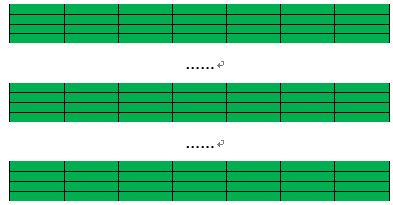
\includegraphics[width=0.4\textwidth]{photo/TEST-chunk-sector.JPG}
\caption{TEST--A sample of chunk and sector}
\label{TEST-chunk-sector}
\end{figure}

In the $n$ chunks of each stripe, we use $m$ parity chunks, and there are $s \times t$ additional symbols in the remaining $n-m$ chunks for encoding. Our goal is to provide different reliability for important and general data, so we assume that normal data can tolerate damage of up to $m$ chunks, while important data can tolerate damage of up to $m+s$ chunks. Figure \ref{TEST-apcode-74222} shows an example of an approximate code for $n = 7$, $r = 4$, $m = 2$, $t=2$ and $s = 2$.
\begin{figure}[ht]
\centering
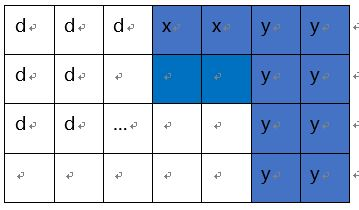
\includegraphics[width=0.4\textwidth]{photo/TEST-apcode-74222.JPG}
\caption{TEST--A sample of Approximate Code with n = 7, r = 4, m = 2, t=2 and s = 2.}
\label{TEST-apcode-74222}
\end{figure}

\subsection{Design of Approximate Code}
\subsection{Encoding and Decoding Processes}
\subsection{Proof of Correctness}
\subsection{Properties of Approximate Code}

\section{Evaluation}
\subsection{An Evaluation methodology}
\subsubsection{Erasure Codes in Our Comparisons}
\subsubsection{Platforms and Configurations}
\subsubsection{Metrics}
\subsubsection{Parameters and Assumption in Our Evaluation}


\subsection{Results}
\subsection{Analysis}
Illustrate why Approximate Code achieve high reliability with low cost
\section{Conclusion}
\section*{Acknowledgment}

\bibliographystyle{IEEEtrans}
\bibliography{paper}

\end{document}
